
%%
%% paper.tex
%% V1.0
%% 2015/05/14
%%

\documentclass[conference]{IEEEtran}

\usepackage{graphicx}
\usepackage{caption}
\usepackage{listings}   %% for code syntax
\lstset{breaklines=true, breakatwhitespace=true}
\lstset{basicstyle=\sffamily}
\lstset{basicstyle=\scriptsize}
\hyphenation{op-tical net-works semi-conduc-tor}

\title{Fake Clicks on Video Ads}

\author{
\IEEEauthorblockN{
Sang Yim\IEEEauthorrefmark{1},
Hsiang Yu Yang\IEEEauthorrefmark{2},
Ozan Okumusoglu\IEEEauthorrefmark{3} and
Dipayan Bhattacharya\IEEEauthorrefmark{4}
}
\IEEEauthorblockA{Carnegie Mellon University\\
Email:
\IEEEauthorrefmark{1}smyim@andrew.cmu.edu
\IEEEauthorrefmark{2}heronyang@cmu.edu
\IEEEauthorrefmark{3}ozano@cmu.edu
\IEEEauthorrefmark{4}dbhattac@andrew.cmu.edu
}}

\begin{document}

\maketitle

\begin{abstract}
Keeping accurate account of views on video advertisement is important since it is now being treated as currency~\cite{c17}. In ``pay per click'' arrangement, publisher (owner of a website), hosts an advertisement and receives pay based on how many users view/click on the advertisement~\cite{c17, c18, c19}. The advertisement is provided by the advertiser (business owner) who pays the publishers so that their advertisement can be viewed by users who visit the website owned by the publisher. This has created an incentive for hackers to generate cheap artificial views on advertisement and trick advertisers to pay significant amount of money~\cite{c17, c18}. In this paper, we analyze traffic of fake views generated by hackers on YouTube and Dailymotion videos. Then we wrote a code which was experimented in various ways to mimic the characteristics of traffic generated by the bots and see if YouTube will accept it as legitimate view
\end{abstract}

\IEEEpeerreviewmaketitle

\section{Introduction}
Association of National Advertisers (ANA) has estimated that artificial views on advertisement will cost advertiser 6.3 billion dollars in 2015~\cite{c1}. ANA also concluded that roughly 23\% of views on advertisements are views that are generated by bots and not real internet users~\cite{c1}. The surprising fact is these artificial views are present in not only armature or personal publishing sites but are also in professional sites which are operated by respected businesses such as Ford, Intel, MasterCard, and Wendy’s~\cite{c3}. The guardian news article stated that about 25\% of artificial views happen on premium sites which are in the top 1000 visited sites in the world~\cite{c3}. These facts can imply two things: 1. Publishers can’t stop fake views/clicks alone. 2. Hackers are building sophisticated bots which emulates user characteristic that are tricking the current defense system.

If 25\% of artificial views happen on premium sites, this means the other 75\% are on armature or non-premium sites. Although it is unclear what defense systems the premium sites are using to defend against fake views, it is clear that the publishers alone can’t stop fake views by themselves. In a recent study in 2014, 181 real video advertisements were observed over 60 days~\cite{c19}. The research found that 23\% of the views of advertisements came from bots. 67\% of the fake views came from residential homes and 58\% were using Microsoft Explorer 6, which has been discontinued since 2008~\cite{c19}. These facts imply that the hackers are infecting vulnerable computers and planting bots to generate artificial views on various advertisements. Indeed this was the case with “Operation Ghost Click” in 2011~\cite{c3, c4}. The U.S. FBI captured 6 Estonian Nationals who were installing rogue DNS servers to infect local DNS cache on vulnerable computers around the world. The rogue servers infected 4 million computers in 100 different countries, 500,000 in the U.S., to redirect users to various sites which hosted advertisements that were linked to the 6 Estonians~\cite{c4}. For example, if the infected computer browses “www.microsoft.com”, user would be redirected to a site that is similar to Microsoft’s site but with random advertisements. The 6 Estonians were able to illegally collect 14 million dollars from the advertisers~\cite{c4}.

It is also evident that the bots are getting more sophisticated to evade detection from any current defense system. Research done by TubeMogul found 3 new sophisticated bots in 2014~\cite{c2}. They state these bots can look like a sports fan, upper class user looking to purchase a car, or senior who are looking at gifts for their grandchildren~\cite{c2}. Although the technical details of the new bots were not stated, this is evident in our research as services that claim to generate views for price were successful delivering view counts on videos hosted by YouTube and Dailymotion.

In this paper, we used 4 services that claim to generate view counts on videos hosted by YouTube and Dailymotion. The prices of their services ranged from 3 to 300 dollars and offered view counts from 50 to 50,000. We purchased the cheapest service ranging from 3 to 8 dollars for 500 to 5000 views. Only three services were able to deliver their view counts in span of 2 to 7 days while one service still haven’t deliver as of May 4$^{th}$ 2015. The statistical data from YouTube and Dailymotion were limited; however, we did find some interesting data as well as verify some information that were stated in other research papers about fake views. Lastly, we wrote some programs which mimics the characteristics of traffics that were analyzed from services that generates view counts for monetary payment. Our programs were tested on videos hosted in YouTube.

In the upcoming sections of the paper, we will describe: the services that we used to generate artificial video view counts, information which were analyzed from statistical data gathered from YouTube and Dailymotion, explanation of our program, and the results of the test.

\section{View Count Generating Services}

\subsection{Buildmyviews.org}
The first service that we used was from http://buildmyviews.org. The IP address of this website is 166.62.5.1, hosted by godaddy.com located in Scottsdale~\cite{c6} U.S. The site’s front page is displayed in figure 1 below. It doesn’t look like a premium website but it does look legitimate but not actively managed. This service offered view counts for videos only hosted by YouTube, but they offered 3 different options of view counts.

\begin{itemize}
  \item Option 1: worldwide view, source of the views will vary from countries worldwide.
  \item Option 2: targeted view, source of the views will come from country of choice.
  \item Option 3: high retention view, the views will watch the whole video making the traffic more like a legitimate views from a real internet user.
\end{itemize}

Aside from the view counts, this service also offered to generate comments on YouTube video. This website claims to offer 24/7 customer support via emails and also chat services. The chat services didn’t seems to work as no one replied when we started to use their chat service screen. Moreover, when we sent an email asking about their basic operation on March 2, 2015, we didn’t receive any reply as of April 2$^{nd}$, 2015. However, when we purchase their service of 1000 views for 3 dollars, we did receive a confirmation email from socialwarehouseorg@gmail.com with the name ``Kevin M''.

\begin{figure}
  \centering
  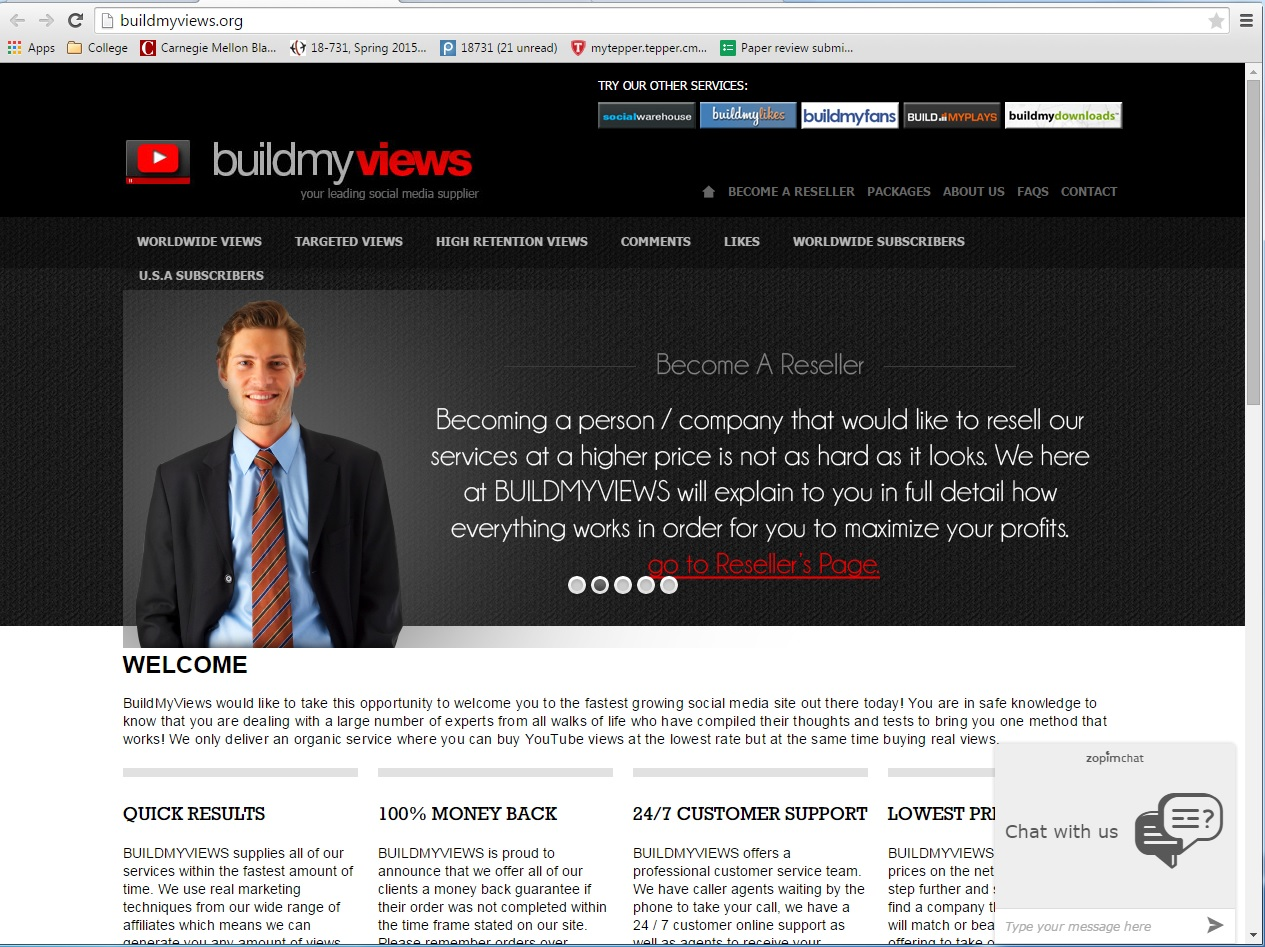
\includegraphics[width=3.0in]{fig1}
  \caption{Front page of Buildmyviews.org}
\end{figure}

\subsection{Dalisocial.com}

The second service that we used was from http://portal.dalisocial.com/. The IP address of this website is 104.24.112.186, hosted by CloudFlare, Inc. located in San Francisco U.S. We needed to register before using the service but we used a random name and an email to get into the site. Email confirmation wasn’t needed and this site didn’t looked professionally managed. However, it offered services across different social media sites. This site offered but not limited to:

\begin{itemize}
  \item Generate ``likes'' on Facebook
  \item Generate ``followers'' on twitter \& Instragram
  \item Generate ``views'' on YouTube
  \item Generate ``plays'' on Soundcloud
\end{itemize}

The Dalisocial site did not offer granular services like buildmyviews.org. For example, it just offered one option to purchase 5000 YouTube views for 7 dollars within 3 days. We noticed the most of the link on the site didn’t work. For example, nothing happened when we clicked the ``Contact Us'', ``About Us'', and ``Blog'' link. The only link that worked was the ``Login'' which directs to a page to purchase services. We did receive an email when we registered and purchase their service of 5000 views for 7 dollars. The email was from noreply@dalisocial.com.

\begin{figure}
  \centering
  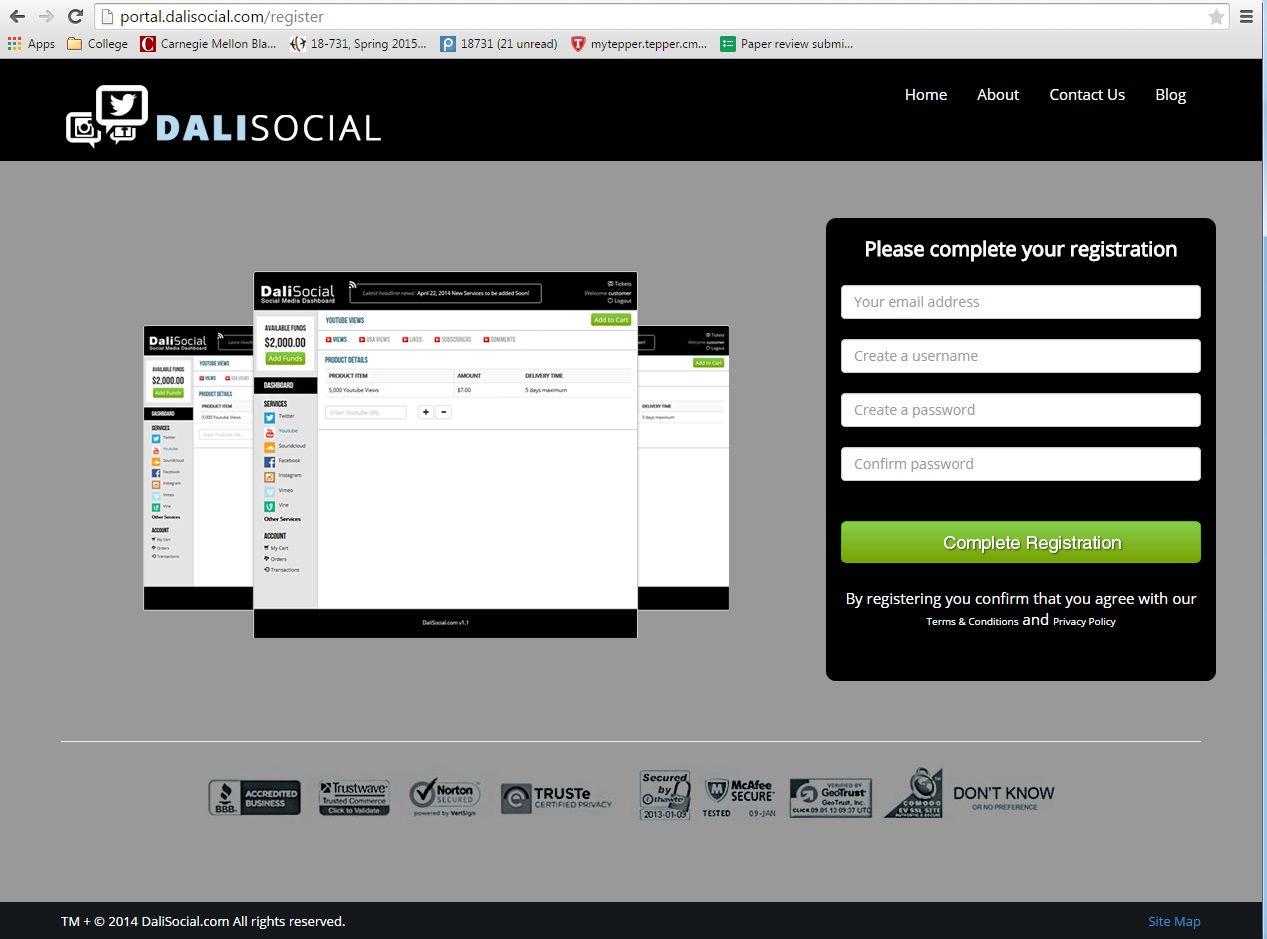
\includegraphics[width=3.0in]{fig2}
  \caption{Front page of DaliSocial.com}
\end{figure}

\subsection{Socialwarrior.net}

The third service that we used was from http://socialwarrior.net. The IP address of this website is 199.188.200.14, hosted by Namecheap, Inc. located in Atlanta, U.S. This site was by far most professional and actively managed. All of the links worked and offered all services that were offered from buildmyviews.org and dalisocial.com. For example, it offered granular option of YouTube views as well as generating “likes” and “followers” on social media sites such as Facebook, twitter, soundcloud, and etc...

We used this service to generate 2000 views for 7.5 dollars on video hosted by YouTube as well as 500 views for 5 dollars on a video that is hosted by DailyMotion.com. And of course, we did received a confirmation order email with tracking number. The most surprising about this site is that they admit that they are generating fake clicks, views, and followers. This is depicted on their ``About'' page and the screen shot displayed in Figure 3 below.

\begin{figure}
  \centering
  
\includegraphics[width=3.0in]{fig3a}
  \caption{``About'' page of SocialWarrior.net}
\end{figure}

\begin{figure}
  \centering
  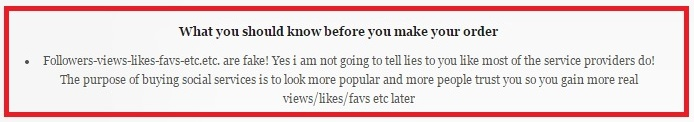
\includegraphics[width=3.0in]{fig3b}
  \caption{The larger screen shot of the red box}
\end{figure}

\subsection{Scopecompany.com}

The last service that we used was from http://www.scopecompany.com. The IP address of this website is 209.59.134.1, hosted by Liquid Web. located in Lansing, U.S. Based on the site, the company states that they are located in New York, US; Mansoura, Egypt; as well as Tokyo, Japan. Aside from generating views on social websites, they offer web service solutions such as web design and development to include specific graphic services.
We used this service to generate 1000 views for 8 dollars on video that is hosted on Dailymotion.com. We did receive a confirmation order email with a tracking number. However, we are yet to see any view counts generated on our target video. We have sent an email acquiring the status of our order but have not receive any reply since May 4$^{th}$, 2015. The website states they 100\% safe and will always deliver within 1 to 5 days.

\begin{figure}
  \centering
  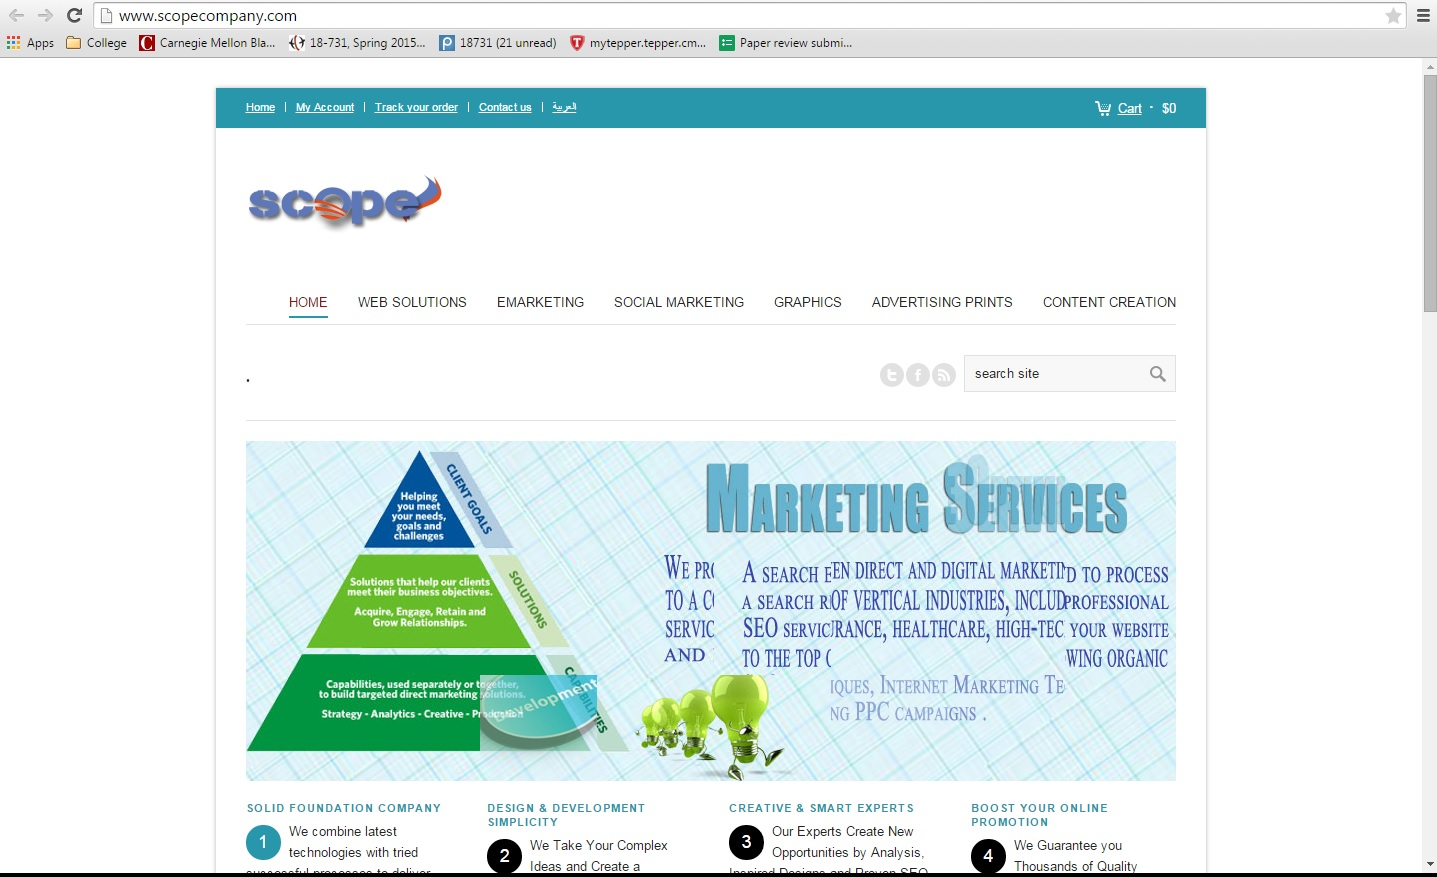
\includegraphics[width=3.0in]{fig4}
  \caption{Front page of Scopecompany.com}
\end{figure}

\section{Traffic Analysis}

In this section, we analyzed data which was generated by the 3 services, since one vendor failed to deliver, that we mentioned in section III. We uploaded 4 different videos: 3 in YouTube and 1 in Dailymotion. All videos were about 60 seconds long and each were tested using different services. Since we can only use statistical data provided by YouTube and Dailymotion, there was limitation of data which could be observed and analyzed. For example, we couldn’t observed the exact IP address but just the general physical location. However, we were able to observe key information such as average duration watched, method of access, what OS was used, and the view counts per day; to come up with the following analysis:

\subsection{Buildmyviews.org}
We bought 1000 views on video hosted in YouTube, which buildmyviews.org delivered within 48 hours. The figure below depicts the representation of view sources by countries.

\begin{figure}[h]
  \centering
  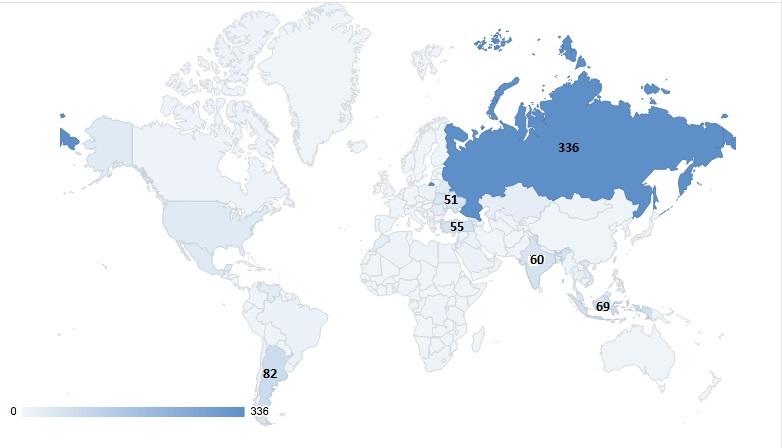
\includegraphics[width=3.0in]{fig5a}
  \caption{Map representation of view source}
\end{figure}

\begin{figure}[h]
  \centering
  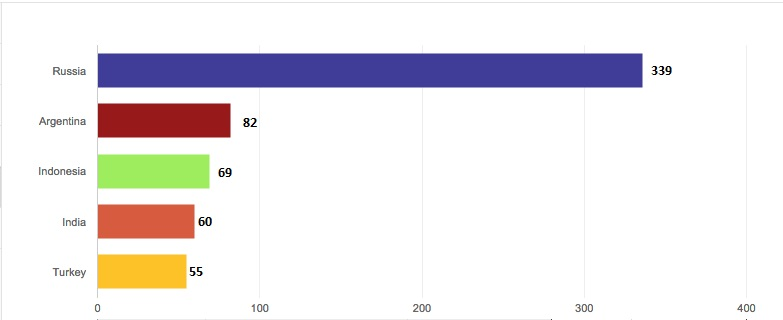
\includegraphics[width=3.0in]{fig5b}
  \caption{The top 5 countries}
\end{figure}

\subsubsection*{Observations}

\begin{enumerate}
  \item The largest chunk of views have been received from Russia (26\%) followed by Argentina (6.4\%), Indonesia (5.4\%), then India (4.7\%).
  \item Average view duration is between 41 to 43 seconds.
  \item There were many ways to view videos on YouTube to include advertised suggested links and through other host sites~\cite{c20}. All of the views generated by the bots are from ``YouTube watchpage'' that is, by typing the URL address or clicking on a link that leads directly to the video on YouTube.
  \item All views used Blackberry OS.
\end{enumerate}

\subsubsection*{Conclusions}

\begin{enumerate}
  \item The services is using same type of bot given the view length time was constant between 41 to 43 seconds, all used Blackberry, and same access method.
  \item The bots are most present in Russia as it showed the most view sources. We are assuming the IP was not spoofed as it is very difficult.
  \item Bots viewed the video for constant duration. This could help us distinguish between the legitimate views from bot generated views.
  \item Bots from buildmyviews.org can only view videos by directly accessing the URL link. The bots are not sophisticated enough to vary their viewing methods such as using advertised links.
  \item might be large amount of comprised Blackberry devices around the world~\cite{c12, c13}; however, the bots might be modifying the traffic to disguise their real operating system.
\end{enumerate}

\subsection{SocialWarrior.net}

We bought 2000 views on video hosted in YouTube and 500 views on video hosted in Dailymotion. Socialwarrior.net delivered the views on YouTube within 48 hours; however, it took about 7 days to deliver 500 views on Dailymotion. For video hosted in Dailymotion, the only statistical data observed was the time (by minute), which the view were generated. We used Dailymotion for this exact purpose since YouTube only provide views by day and not by exact time. The figure below depicts the representation of view sources by countries (Video hosted on YouTube only).

\begin{figure}[h]
  \centering
  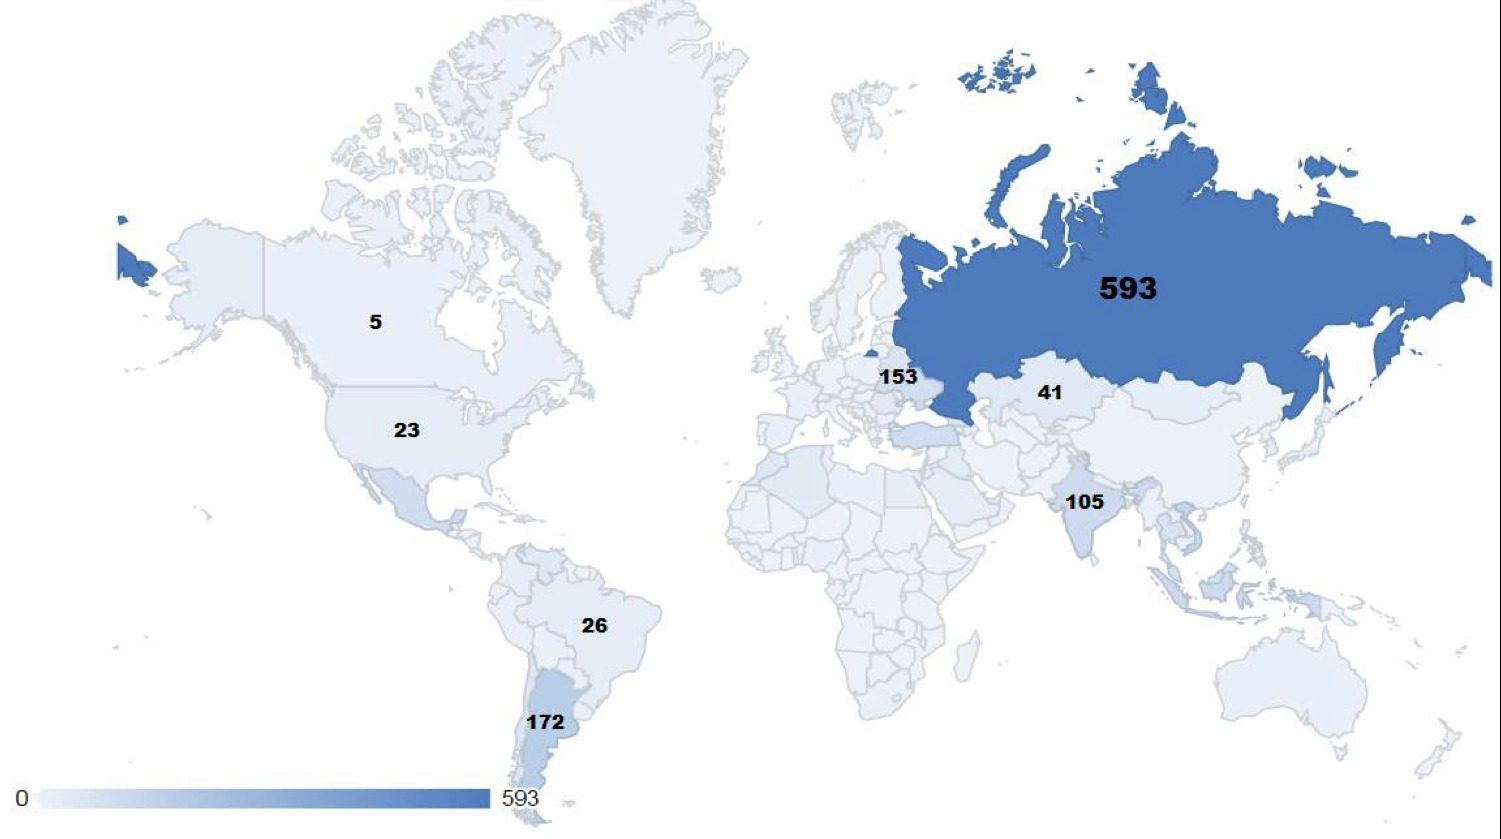
\includegraphics[width=3.0in]{fig6a}
  \caption{Map representation of view source}
\end{figure}

\begin{figure}[h]
  \centering
  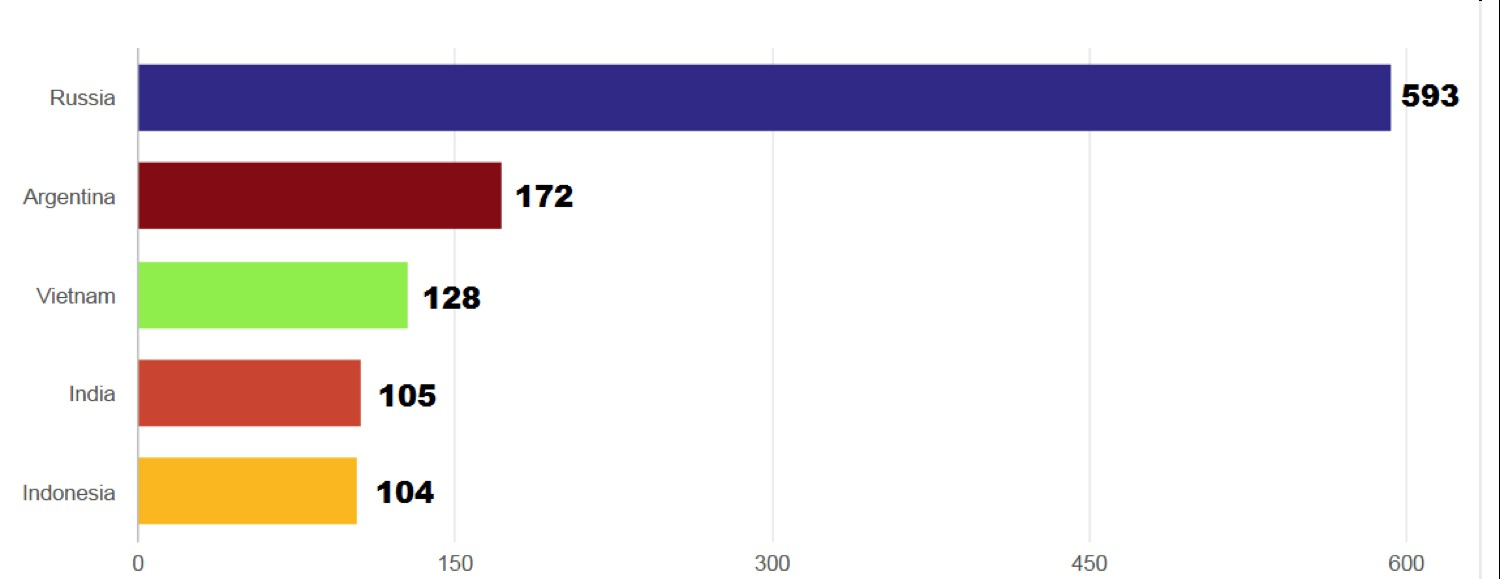
\includegraphics[width=3.0in]{fig6b}
  \caption{The top 5 countries}
\end{figure}

\subsubsection*{Observations}

\begin{enumerate}
  \item SocialWarrior.net used same or very similar type of bot from Buildmyviews.org to generate the views as we observe similar characteristics.
  \begin{itemize}
    \item Russia accounts for the highest number of views followed by Argentina.
    \item View length was different but still constant at 57 seconds.
    \item Used the same access method: ``YouTube watchpage''.
    \item All views used Blackberry OS.
  \end{itemize}
  \item The bots have viewed almost whole duration of the video hosted in YouTube, 57 seconds.
  \item It took significantly longer to deliver view counts on video hosted by Dailymotion. The 2000 view counts on YouTube was delivered in 48 hours while it took about a week to deliver view counts on Dailymotion.
  \item The view counts on Dailymotion wasn’t generated systematically. We did not find a definite pattern but views were generated once or twice every 7-14 minutes for few hours, then go into a long pause, then start generating views again every 7-14 minutes.
\end{enumerate}

\subsubsection*{Conclusions}

\begin{enumerate}
  \item As already mentioned, SocialWarrior.net may used same or very similar type of bot from Buildmyviews.org as we observed similar characteristics.
  \item Assuming SocialWarrior,net and Buildmyviews.org used the same type of bot, the bots are flexible to view the whole or just part of the video.
  \item YouTube and Dailymotion use different system to count views. That is why it took only 48 hours to deliver 2000 views on YouTube while it took about a week to deliver only 500 views on Dailymotion.
  \item SocialWarrior.net used different methods to generate views on YouTube and Dailymotion. On Dailymotion, only the time can be observed, we didn’t receive other data such as the source locaton, OS, and access method. However, based on the time data, SocialWarrior.net could have used real users to generate view counts on Dailymotion, as it isn’t hard to generate 500 views in period of 7 days.
\end{enumerate}

\subsection{Dalisocial.com}

We bought 5000 views on video hosted in YouTube, which Dailsocial.com delivered within 72 hours. The figure below depicts the representation of view sources by countries.

\begin{figure}[h]
  \centering
  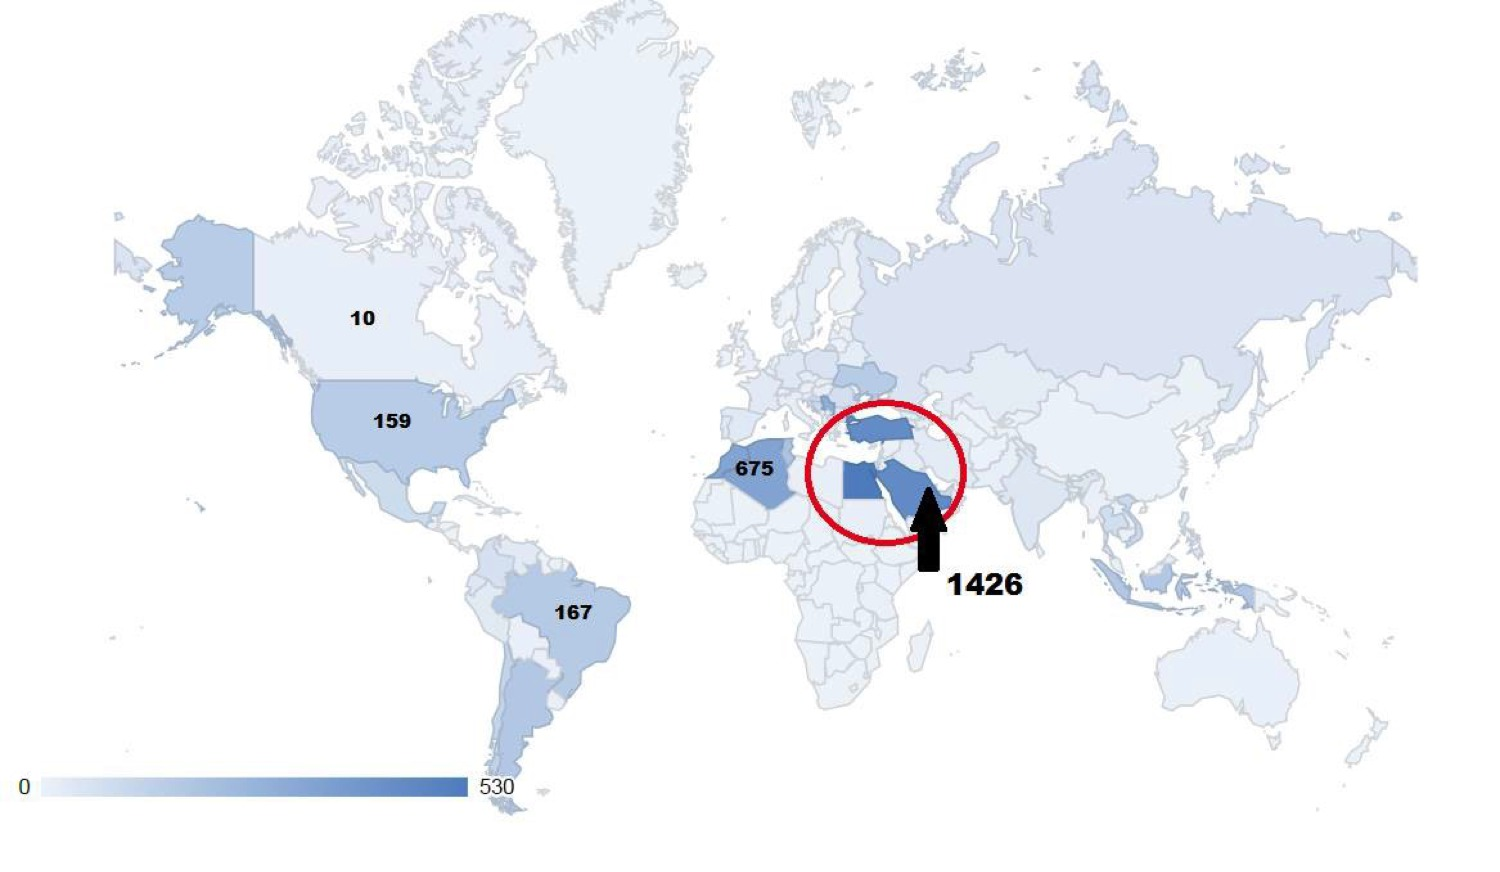
\includegraphics[width=3.0in]{fig7a}
  \caption{\label{7a} Map representation of view source}

\end{figure}
\begin{figure}[h]
  \centering
  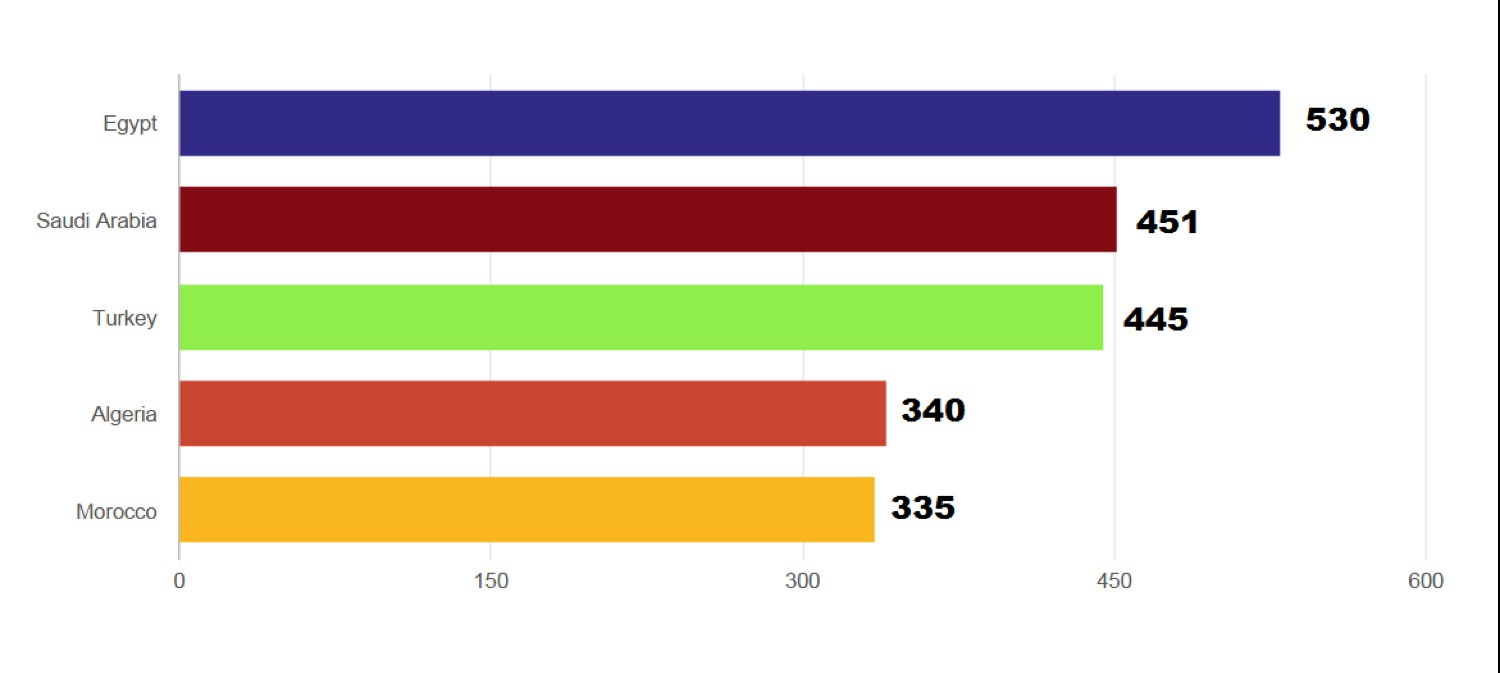
\includegraphics[width=3.0in]{fig7b}
  \caption{The top 5 countries}
\end{figure}

\subsubsection*{Observations}

\begin{enumerate}
  \item The view sources were evenly distributed especially in the Middle East: Egypt, Saudi Arabia and Turkey (Fig. \ref{7a}).
  \item All bots viewed the entire video, 60 seconds.
  \item 51\% of views are from “YouTube homepage”, meaning, the video was accessed via link suggested by YouTube.  This is only possible if you have a YouTube account~\cite{c21}.
  \item 49\% of bot views are direct views, same method as previous 2 services used.
  \item 99\% of the traffic is from computers, mostly from Windows OS, but MAC and Linux also had small presence (less than 2\% each).
  \item 18 out of 5000 views from gaming consoles, from Saudi Arabia and Germany.
  \item 17 out of 5000 views from mobile devices; Android and IPhone but no Blackberry.
\end{enumerate}

\subsubsection*{Conclusions}

\begin{enumerate}
  \item Dalisocial.com used different type of bot than Buildmyviews.org and SocialWarrior.net, as it showed different characteristics:
  \begin{itemize}
    \item Different source concentration, Middle East vs. Russia
    \item 2 different access methods vs. 1 access method
    \item Various OS vs. one Blackberry OS
  \end{itemize}
  \item Bots used by Dalisocial.com were more sophisticated as the traffics seem like a real users. They were able to access the video in different ways, view the whole length, and used various different devices/OS.
  \item The bots used by Dalisocial.com are most concentrated on Middle East as top 5 sources are from that area.
  \item The bots somehow made Google accounts to access the video via link suggested by YouTube homepage. This type of access is only available with having a Google account, thus it shows the high sophistication level of these bots~\cite{c21}. There is also a possibility that Dalisocial.com used a real users to generate the views; however, it is highly unlikely that they are connected with hundreds of users over 20 different countries who would collaborate to provide this type of services for \$7.
\end{enumerate}

\subsection{Summary of our findings}

Based on the observations generated by 3 different services, we summarize the following:

\begin{enumerate}
  \item Not all traffics from the bots are counted as views. Which means, there is no definite way for the services to provide the exact number of views as required by the customers. It was found all 3 services overprovided the number of views requested. This implies that there is a central command system which turns the bots on to generate the traffic, then turns them off when the view counts are roughly met.
  \item There are at least 2 different type of bots used to generate artificial view counts. This is obvious as Dalisocial.com used different bots than the other two services. We assume that Buildmyviews.org and SocialWarrior.net used the same type of bot since the characteristics were very similar as well as services offered by the two websites.
  \item There is a possibility that many Blackberry devices are infected with bots that are being used to generate artificial view counts. According to PMR, there are at least 100,000 Blackberry devices in Russia since 2011~\cite{c13}, which bot type of malware was discovered on mobile devices, including Blackberry, around the same time~\cite{c12}.
  \item The businesses which offer to generate view counts on social media sites are not professionally maintained. One of the services did not deliver the view counts after taking the payment from our pre-paid credit card account. Moreover, all 4 services did not reply to our calls and emails that were provided on their customer care site.
\end{enumerate}

\section{Code}

\subsection{YouTube view count system}

Here we tried to use our own code to generate artificial view counts on videos hosted in YouTube. Before writing the code, we studied how YouTube view counting system works. The following is the list of what we’ve learned:

\begin{enumerate}
    \item YouTube has many distributed log servers which reports to one centralized server that manages all view counts~\cite{c11}.
    \item When a video hosted in YouTube view count reaches 301, all additional views are verified by the centralized server~\cite{c11}. The verification process could take few hours to several days. Thus, view count might be stuck on 301 views.
    \item After view count reaches 301, YouTube discriminates views from same source IP in period between 6 to 8 hours~\cite{c11}. For example, if one user (with same IP) views the same video 500 times in 6 hours, the actual view count accepted by YouTube might only be 3 to 5.
\end{enumerate}

\subsection{Browser interaction with YouTube Player}

Here we explain the interaction between the client browser and videos hosted in YouTube. We learned the interaction by observing the source HTML code on our browser when loading videos on YouTube. This understanding is necessary as we used this mechanism to write the code to generate fake views on YouTube.

\begin{enumerate}
  \item When client browser tries to view a video from YouTube, it sends HTTP GET Request to YouTube service, then loads the following HTML code to create a blank video player:
  \begin{lstlisting}[frame=single, language=html]
<div id="player-api" class="player-width player-height off-screen-target player-api" tabIndex="-1">
</div>
  \end{lstlisting}
  \item The JavaScript code within the HTML file loads the YouTube player (Adobe Flash Player) into the client’s browser.
  \begin{lstlisting}[frame=single, language=html]
<script>
  var ytplayer = ytplayer || {};
  ytplayer.config = { "min_version":"8.0.0", "url":"https:.../watch_as3.swf"
  ...
</script>
  \end{lstlisting}
  \item Lastly, the YouTube sends necessary data to the browser so the YouTube video player can load the specific video the browser requested. Then the video is played automatically and at this point, it should generated a view count.
  \begin{lstlisting}[frame=single, language=html]
<embed name="movie_player" id="movie\_player" type="application/x-shockwave-flash" src="https:.../watch\_as3.swf" allowscriptaccess="always" bgcolor="#000000" allowfullscreen="true" ...>
  \end{lstlisting}
\end{enumerate}

\subsection{Our code to generate views on YouTube}

In order to generate YouTube views, we've tried publically available Javacript codes: PhantomJS and SeleniumHQ. PhamtonJS didn’t work to generate views on YouTube since it doesn’t support Adobe Flash Player; SeleniumHQ, however, was successful as it was tested on normal client machines as well as Ubuntu Server.

Since we didn’t need the browser popup displaying YouTube videos, we used Xvfb (Virtual framebuffer X server for X Version 11) to buffer screen display in the background while taking snapshots for information analysis and debugging purposes.

The following are the steps of execution of our code to generate views on videos hosted in YouTube:

\begin{enumerate}
  \item Start Xvfb to buffer screen display instead of popping up browser GUI.
  \item With SeleniumHQ library, the script loads browser driver based on its deploying platform. In our experiment, we use Firefox on Ubuntu OS.
  \item Request the target video from YouTube page, then sleep for short random duration then request it again.
  \item Close the page and the driver.
\end{enumerate}

\begin{figure}
  \centering
  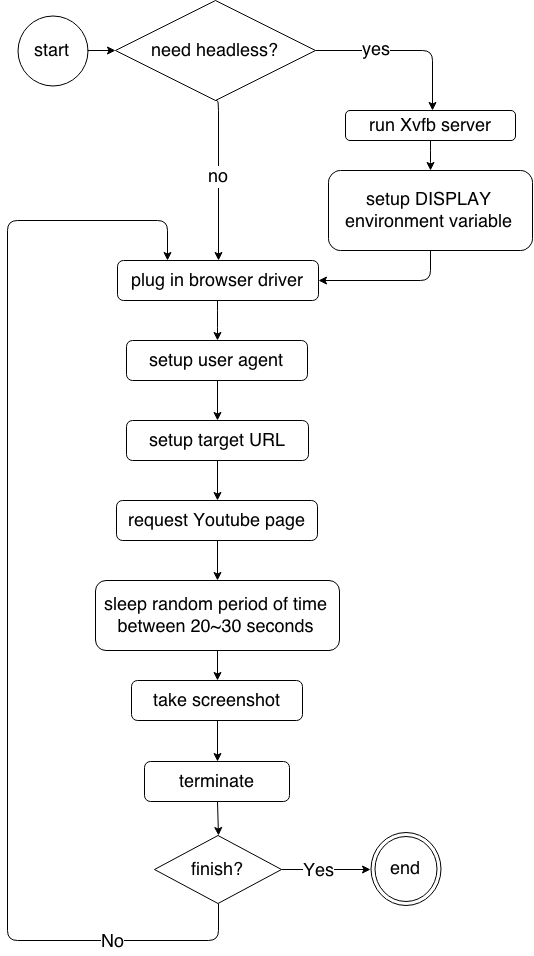
\includegraphics[width=3.0in]{flowchart}
  \caption{Flowchart of our fake click generating code}
\end{figure}

Refer to our Github repository for the actual code (https://github.com/heronyang/youtube\_fake\_view). With our code, we were able to generate at least 301 view counts on videos hosted in YouTube, using one machine with one user agent. This is because YouTube view counting system analyzes the view counts after 301 and determined that the views generated by our code isn’t from a real user. In our next section, we explain how we used our code in various ways to implement more unique IP addresses, user agents, and VPN connections to pass the 301 views on videos hosted in YouTube.

\section{Experiments}

\subsection{Incorporating multiple user agents}

In HTTP, a user agent is a string that is inserted with initial HTTP GET request for content negotiation. User agent string identifies: application type, operating system, software vendor, and software revision number that are being used by the requestor~\cite{c16}. With this information, the service provider, i.e. Web Server, sends contents that are compatible based on user agent information~\cite{c16}.

We are assuming YouTube view counting system checks user agent information since this could be an obvious indicator to detect bot traffic. For example, it is highly unlikely that a video suddenly gets viewed 1000 times with the exact same user agent string. There are too many different OS/browser combination available for 1000 random users to have the same user string, and since one user wouldn’t constantly view the same video 1000 times, this could be an obvious sign of bot traffic. Therefore, we tested our code using 526 different user agent strings to see if we can generate more than 301 artificial view counts on video hosted in YouTube.

We modified our code to use a specific user agent string or parse it from a file that has a list of different user agent strings. Please refer to our Github repository for full description of different parameters that could be used.

We created an agents.txt file which contains 526 different user agent strings. Then we executed the code by typing the following command:

\begin{lstlisting}[frame=single, language=bash]
python fake_user.py -f user agents.txt -t YOUTUBE_URL
\end{lstlisting}

Setup environment where this experiment was executed:
\begin{itemize}
  \setlength\itemsep{-0.1em}
  \item OS: Ubuntu 14.01 Server
  \item Duration: From April 28$^{th}$ 2030-2300 (3hr, 30min)
  \item Public IP: 172.31.20.23
  \item User agent: 526 different user agents
  \item 150-200 views every hour
\end{itemize}

\subsubsection*{Findings}
\begin{itemize}
  \setlength\itemsep{-0.1em}
  \item View count quickly generated to 301 in few hours but unchanged as of May 3rd, 2015.
  \item User agent information can easily be changed, thus there is probably no mechanism to verify if user agent string actually matches the source OS/browser used.
  \item For user agents with BlackBerry strings, YouTube sent pure HTML files with link to RTSP stream protocol instead of adobe flash player.
\end{itemize}


\subsection{Incorporating more IP addresses via Cloud Service}

Here we used multiple public IP addresses with our code to pass the 301 view threshold on video hosted by YouTube. Considering only IPv4, there are little less than 4 billion public IP addresses available in the world.

Again, we are assuming YouTube view counting system checks source public IP address since this information could be used to detect bot traffic. A video with 1000 views should have multiple public source IP addresses since users are geographically separated and use different ISPs. Although many users share same publish IP address, it is highly unlikely that all 1000 real views came from one public IP address out of 4 billion. Therefore, we used Amazon’s instances to incorporate 5 different IP addresses when executing our artificial view count generating code.

Setup environment where this experiment was executed:
\begin{itemize}
  \setlength\itemsep{-0.1em}
  \item OS: 5 Amazon Instances (t2.micro)
  \item Duration: From April 29$^{th}$ 1730~2050 (3hr, 20min)
  \item Browser: Firefox 37.0.2
  \item Each instance views 60~120 views every hour
\end{itemize}

\subsubsection*{Findings}
\begin{itemize}
  \setlength\itemsep{-0.1em}
  \item View count quickly generated to 301 within one hour but unchanged as of May 4$^{th}$ 2015.
  \item 5 public IP addresses isn’t enough to pass 301 view count.
\end{itemize}


\subsection{Incorporating more IP addresses via TOR}

The Onion Router provides user anonymity on the Internet through encryption and using 3 random node connections between the source and the destination~\cite{c14}.

We thought about using TOR because it can incorporate many public IP addresses using different TOR exit nodes with our code. If the TOR daemon is configured to setup a new circuit every time our code views a YouTube video, we can use hundreds of different IP addresses since there are around 1000 different exit nodes available~\cite{c15}.

Setup environment where this experiment was executed:
\begin{itemize}
  \setlength\itemsep{-0.1em}
  \item OS: MAC OS X v10.10
  \item Duration: From April 30th 1730-0330 (10 hrs)
  \item Browser: Firefox 37.0.2
  \item 50-60 views every hour
\end{itemize}

\subsubsection*{Findings}
\begin{itemize}
  \setlength\itemsep{-0.1em}
  \item View count is still stuck at 301.
  \item Source IP is visible via flash browser plugin~\cite{c14}. This means that YouTube knows where the actual request is coming from; thus, anonymity isn’t possible using TOR when viewing videos in YouTube.
\end{itemize}


\subsection{Incorporating VPN connections}

Virtual Private Network is a connection that extends to another network through public network connection~\cite{c23}. Many higher institutions offer VPN service so students and staff can connect to the institution’s network from home or other geographic locations.

There are many free VPN connections available and hence many users use VPN for security and privacy~\cite{c24}. Since many users use popular VPN services, we assume that YouTube knows the VPN public IPs and think multiple users can be associated with one VPN IP address. We tested this hypostasis with our code and see if it can break the 301 view count on YouTube videos.

Setup environment where this experiment was executed:
\begin{itemize}
  \setlength\itemsep{-0.1em}
  \item OS: Ubuntu 14.04 LTS
  \item Duration: From May 1$^{th}$ 1730-2130 (4 hrs)
  \item Browser: Mozilla/5.0
  \item 120-180 views every hour
  \item VPN: Security KISS Services
  \item IP address: 217.147.83.21 (UK)
\end{itemize}

\subsubsection*{Findings}
\begin{itemize}
  \setlength\itemsep{-0.1em}
  \item View count is still stuck at 301.
  \item Using popular VPN connection doesn’t matter.
\end{itemize}

\subsection{Summary of Experiments}

We were able to generate 301 view count on videos hosted by YouTube using our code in various different ways. However, we were not able to pass the 301 view count as of May 4$^{th}$ 2015. We also like to mention that we used combination of our experiments on one video hosted by YouTube. For example, we used VPN connection and 5 Cloud instances using multiple user agents. The result was similar as we were able to generate view count up to 301 views but no more.

Lastly, YouTube counting system isn’t perfect as it proven to allow both false positive and false negative view counts in our research. We were able to prove it allows false positive view counts by using the 4 services mentioned in section 2 \& 3. Moreover, for the videos that were stuck on 301+ views, we view the same videos manually and see if the view count will go over 301. The view counts didn’t change even after we manually view the videos; therefore, we assume that YouTube’s counting
system is also vulnerable to false negative view counts.

\section{Related Works}

Fake view on video advertisement is relatively new; thus, not many published research are available. However, there is a researched conducted by Cornell University, where they partnered with Tencent Video and were able to collect much data on real video advertisements~\cite{c5}. They came up with the idea to calculate entropy value base on captured traffic. It distinguishes real and bot traffic based on the entropy value where lower the number, it more likely a bot. The authors stated that
their entropy value system was 98\% accurate distinguishing real to fake views on video advertisements~\cite{c5}; thus, we assume YouTube is using a similar system. As mentioned before, YouTube stops the count at 301 views and analyzes the traffic before granting any more view counts. This closely fits into the Cornell’s entropy system, where captured traffic is carefully analyzed to distinguish between real and fake views on video advertisements.

Similar research was done by UC San Diego, University of Texas, and Microsoft where they focused to catching spam clicks on online advertisements~\cite{c18}. This research used around 10 ethical publishers as a baseline to calculate the Return On Investment (ROI) value, then assume that spam clickers have higher ROI value~\cite{c18}. This research is interesting since it focuses the heart of the issue where money derived from artificial views create incentives for hackers.

Lastly, another research was done to analyze the spam eco-system~\cite{c18}. In this research, the authors carefully analyzed how the spam services are provided and found a bottleneck (payment system) that can be used to stop the whole spam eco-system~\cite{c18}. Key information found in this research can be related to the 4 services that we used on section 2\&3. Thus, future research should be conducted if the services which provide artificial views on videos has the same bottleneck as the
spam eco-system.


\section{Conclusions}

In our research, we used view count generating services to analyze bot traffic which artificially views YouTube and Daily Motion videos. We found that bots are widely distributed, very sophisticated, and flexible. In our second part of the research, we wrote our own artificial view count generating code and test it in various ways to simulate the bots that were being used by the artificial view generating services.

We find it difficult to emulate the bots that are being used by the 3 services we used on this research for 2 reasons:

\begin{enumerate}
  \item The data provided by YouTube isn’t enough to technically evaluate the characteristics of artificial view generating bots. The limitation of the data is already mentioned on Traffic Analysis section of the research. Perhaps, we could request granular statistical information from YouTube to provide the following:
  \begin{itemize}
    \item Exact time the views were generated
    \item The public source IP address
    \item User agent string for each view
  \end{itemize}
  \item We didn’t have enough resources. As observed from the 3 artificial view generating services, bots were present from at least 20 different countries which was able to pass the 301 view count on YouTube video within 48 hours. Perhaps if we can partner with other universities around the world, we can run our code in various places to see if we can also pass the 301 view count.
\end{enumerate}

\bibliographystyle{IEEEtran}
\bibliography{cite}

% that's all folks
\end{document}
